\documentclass{article}[18pt]
\usepackage{../../../../../format}
\lhead{Bioinformatics}


\begin{document}
\begin{center}
\underline{\huge Question 2}
\end{center}
\begin{tabular}{|c|c|c|c|c|c|c|}
	\hline 
	& A & B & C & D & E & F \\ 
	\hline 
	A & 0 & 15 & 24 & 29 & 25 & 37 \\ 
	\hline 
	B & 15 & 0 & 32 & 31 & 23 & 43 \\ 
	\hline 
	C & 24 & 32 & 0 & 30 & 43 & 49 \\ 
	\hline 
	D & 29 & 31 & 30 & 0 & 45 & 57 \\ 
	\hline 
	E & 25 & 23 & 43 & 45 & 0 & 55 \\ 
	\hline 
	F & 37 & 43 & 49 & 57 & 55 & 0 \\ 
	\hline 
\end{tabular} \\
The edge weight between A and B is the smallest, so merge them
\vspace{1cm}
\\
\begin{tabular}{|c|c|c|c|c|c|}
	\hline 
	& AB & C & D & E & F \\ 
	\hline 
	AB & 0 & 28 & 30 & 24 & 40 \\ 
	\hline 
	C & 28 & 0 & 30 & 43 & 49 \\ 
	\hline 
	D & 30 & 30 & 0 & 45 & 57 \\ 
	\hline 
	E & 24 & 43 & 45 & 0 & 55 \\ 
	\hline 
	F & 40 & 49 & 57 & 55 & 0 \\ 
	\hline 
\end{tabular} \\
The edge weight between AB and E is the smallest, so merge them
\vspace{1cm}
\\
\begin{tabular}{|c|c|c|c|c|}
	\hline 
	& ABE & C & D & F \\ 
	\hline 
	ABE & 0 & 33 & 35 & 45 \\ 
	\hline 
	C & 33 & 0 & 30 & 49 \\ 
	\hline 
	D & 35 & 30 & 0 & 57 \\ 
	\hline 
	F & 45 & 49 & 57 & 0 \\ 
	\hline 
\end{tabular} \\
The edge weight between C and D is smallest, so merge them
\vspace{1cm}
\\
\begin{tabular}{|c|c|c|c|}
	\hline 
	& ABE & CD & F \\ 
	\hline 
	ABE & 0 & 34 & 45 \\ 
	\hline 
	CD & 34 & 0 & 53 \\ 
	\hline 
	F & 45 & 53 & 0 \\ 
	\hline 
\end{tabular} \\
The edge weight between ABE and CD is the smallest, so merge them
\vspace{1cm}
\\
\begin{tabular}{|c|c|c|}
	\hline 
	& ABECD & F \\ 
	\hline 
	ABECD & 0 & 48.2 \\ 
	\hline 
	F & 48.2 & 0 \\ 
	\hline 
\end{tabular} 
\\
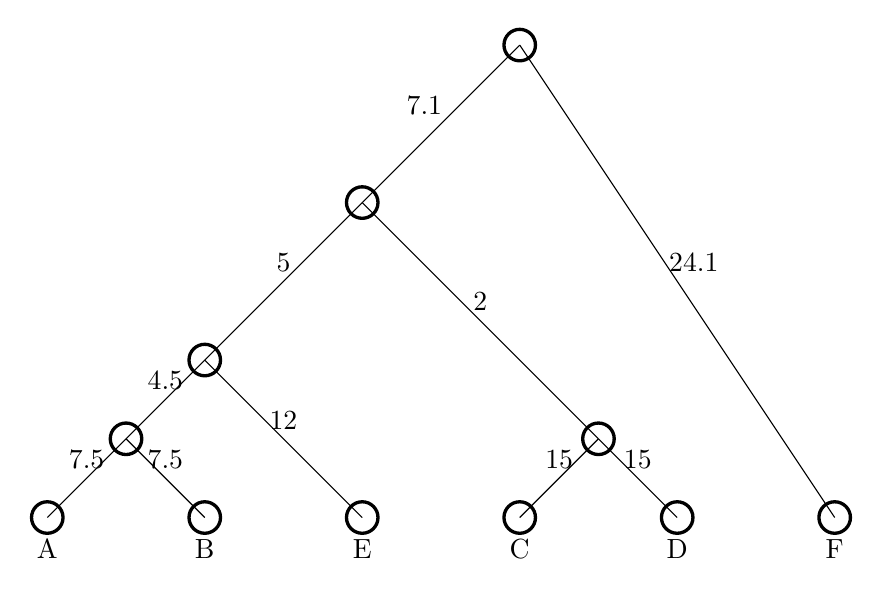
\begin{tikzpicture}[scale=2]
\filldraw[color=black, fill=none, very thick] (0,0) circle (0.1) node[below,yshift=-4]{A} ;
\filldraw[color=black, fill=none, very thick](1,0) circle (0.1) node[below,yshift=-4]{B};
\filldraw[color=black, fill=none, very thick](0.5,0.5) circle (0.1);
\draw (0,0) -- (0.5,0.5) node[pos=0.5,above]{7.5};
\draw (1,0) -- (0.5,0.5) node[pos=0.5,above]{7.5};
\filldraw[color=black, fill=none, very thick](2,0) circle (0.1) node[below,yshift=-4]{E};
\filldraw[color=black, fill=none, very thick](1,1) circle (0.1);
\draw (2,0) -- (1,1) node[pos=0.5,above]{12};
\draw (0.5,0.5) -- (1,1) node[pos=0.5,above]{4.5};
\filldraw[color=black, fill=none, very thick](3,0) circle (0.1) node[below,yshift=-4]{C};
\draw (1,1) -- (2,2) node[pos=0.5,above]{5};
\filldraw[color=black, fill=none, very thick](4,0) circle (0.1) node[below,yshift=-4]{D};
\filldraw[color=black, fill=none, very thick](3.5,0.5) circle (0.1);
\draw (3,0) -- (3.5,0.5) node[pos=0.5,above]{15};
\draw (4,0) -- (3.5,0.5) node[pos=0.5,above]{15};
\draw (3.5,0.5) -- (2,2) node[pos=0.5,above]{2};
\filldraw[color=black, fill=none, very thick](2,2) circle (0.1);
\filldraw[color=black, fill=none, very thick](5,0) circle (0.1) node[below,yshift=-4]{F};
\filldraw[color=black, fill=none, very thick](3,3) circle (0.1);
\draw (5,0) -- (3,3) node[pos=0.5,above,xshift=6]{24.1};
\draw (2,2) -- (3,3) node[pos=0.5,above,xshift=-6]{7.1};
\end{tikzpicture}







\end{document}